\chapter{Experimentos y resultados}\label{chapter:results}

En este capítulo se presentan los experimentos realizados para evaluar el desempeño de la regresión simbólica propuesta en el capítulo anterior y sus resultados.

\section{Consideraciones de la etapa de experimentación}\label{section:experimental_considerations}

El espacio de búsqueda en la regresión simbólica planteada en el anterior capítulo comprende a todos los sistemas de ecuaciones diferenciales donde la cantidad de ecuaciones es definida según los datos, y como se mencionaba la regresión simbólica es un problema NP-difícil por lo que resulta computacionalmente costoso utilizar este método. Por esta razón, se diseñó un marco experimental que fuese factible de ejecutar con recursos limitados. El equipo de cómputo donde se realizaron los experimentos posee las siguientes propiedades.


\begin{itemize}
    \item \textbf{Procesador}: 11th Gen intel i9-11900H @ 2.50GHz
    \item \textbf{RAM}: 40GB
    \item \textbf{Arquitectura}: 64 bits
\end{itemize}

La implementación de la solución se desarrolla en el lenguaje de programación \emph{Python} auxiliado por bibliotecas como \emph{numpy} y \emph{scipy} de código abierto implementadas en el mismo lenguaje.

Cómo métrica se utiliza la función para determinar el costo de una solución definida en la sección \ref{section:solution_cost}. A menores valores de esta métrica implica que el sistema obtenido en la regresión simbólica se ajusta mejor a los datos.

Cada experimento que aparece en la sección \ref{section:experiments} fue realizado 30 veces y se plantea el valor promedio que obtuvo la métrica utilizada en estas 30 ejecuciones del experimento. Además se indica el valor mínimo y máximo que alcanzó la métrica a lo largo de los 30 experimentos.

En la siguiente sección se precisa mejor cómo se generan los datos para realizar los distintos experimentos.

\section{Descripción del marco experimental}

Los experimentos parten de la selección de un modelo conocido $f$, por ejemplo el modelo poblacional SIR:

\begin{align*}
    S' & = - a*I*S     \\
    I' & = a*I*S - b*I \\
    R' & = b*I.
\end{align*}

Este se integra en un intervalo definido y se obtiene un conjunto de puntos que representan el valor de las distintas variables a lo largo del tiempo. Por ejemplo si se integra el modelo SIR con $0 \leq t \leq 20$ se obtienen las curvas en la imagen \ref{fig:SIR}.

\begin{figure}[h]
    \centering
    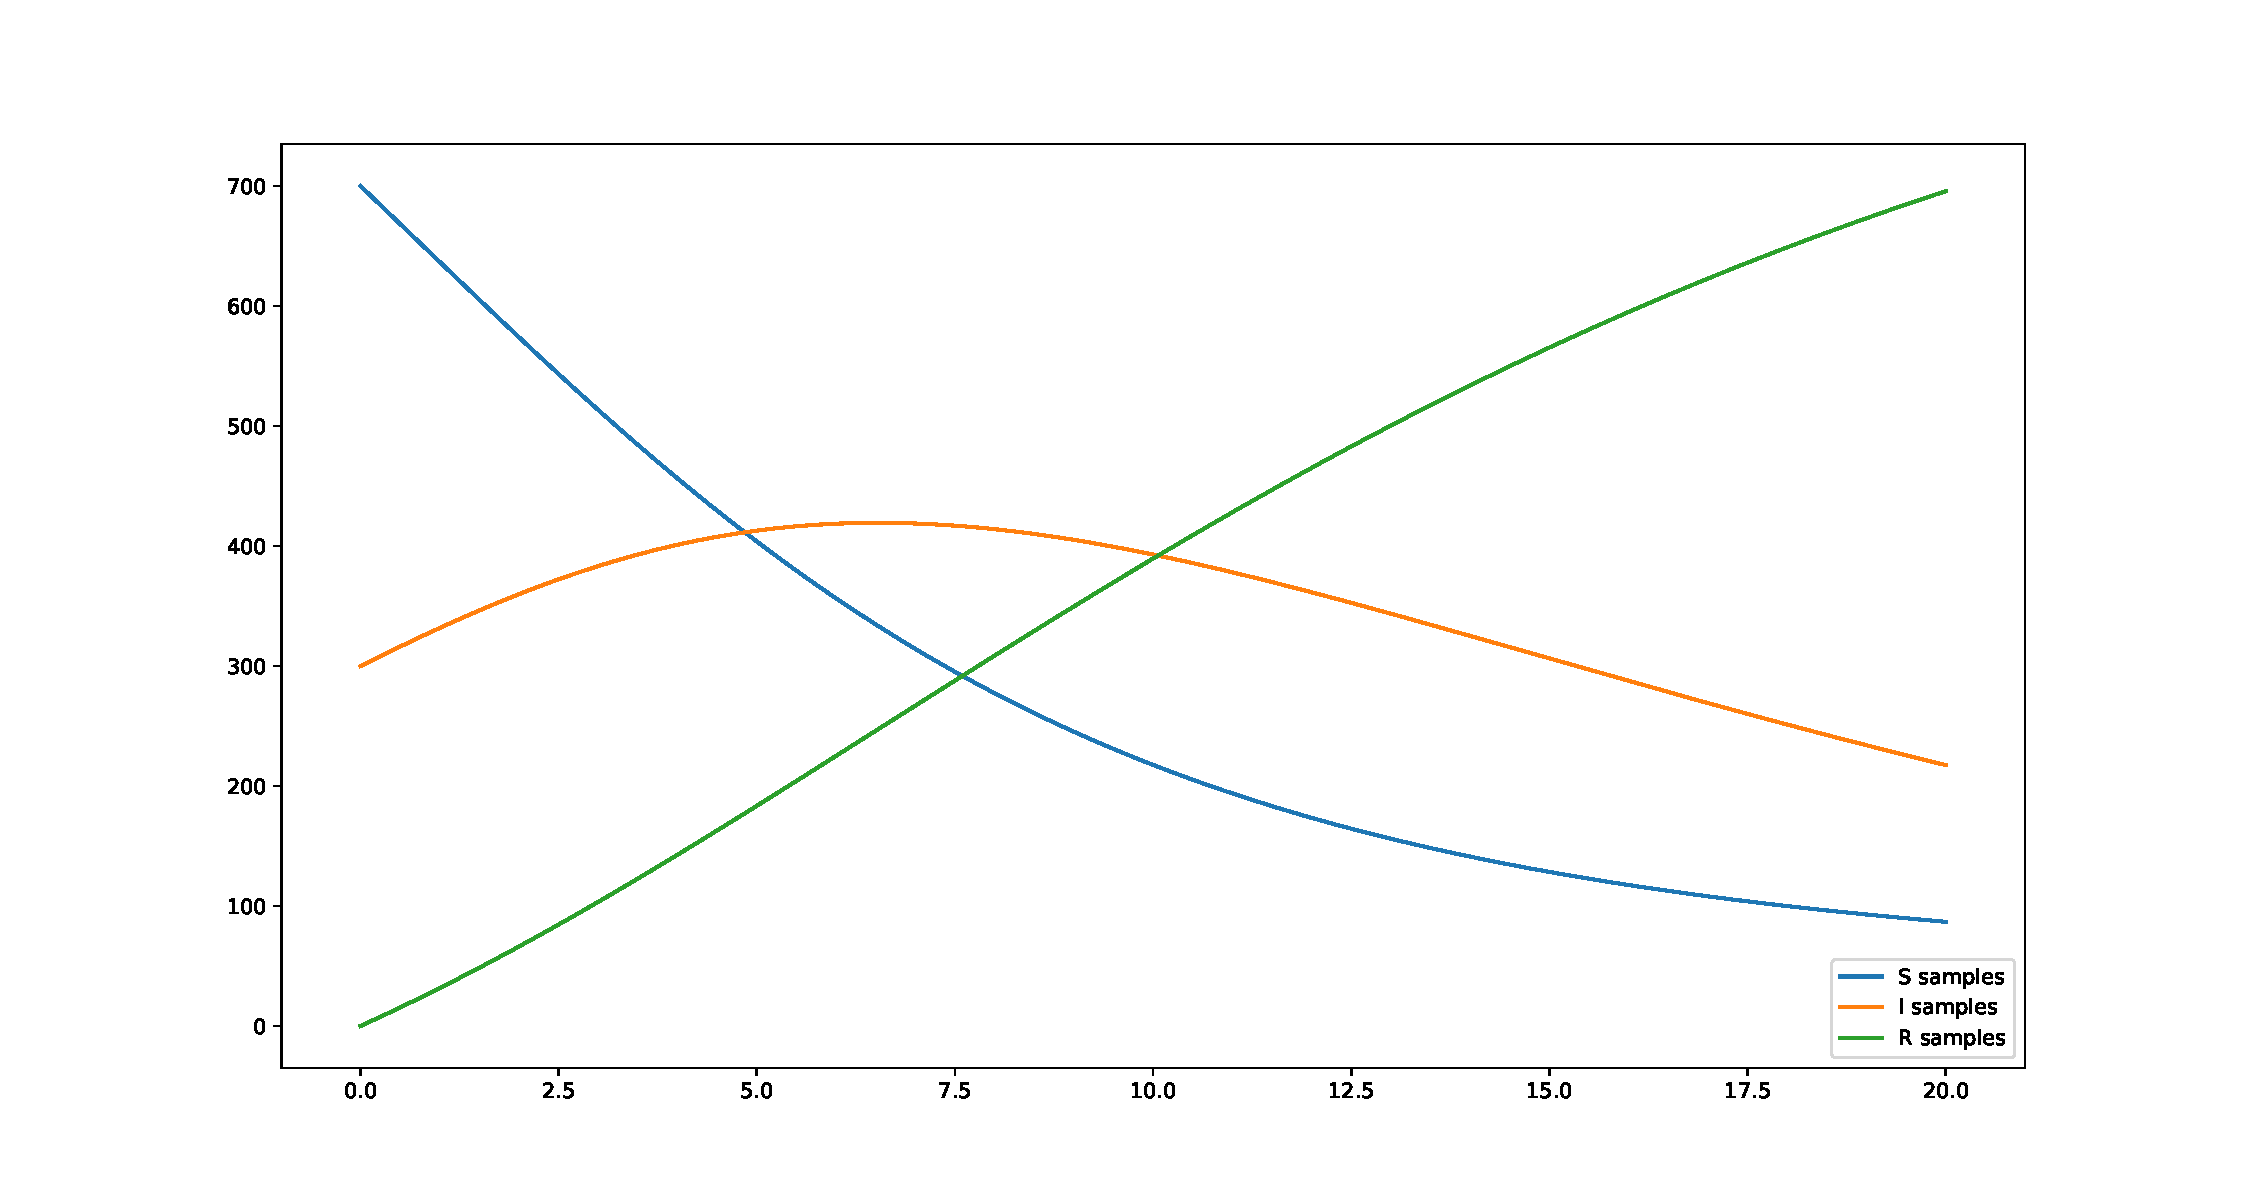
\includegraphics[width=\textwidth]{"figures/SIR.pdf"}
    \caption{modelo poblacional SIR con $a = 0.0003, b = 0.1$.}
    \label{fig:SIR}
\end{figure}

Luego se le agregan distintos valores de ruido a los puntos, este ruido puede tener un valor máximo de 0\%, 5\% o 10\% con respecto a cada muestra. Por ejemplo si escoge como ruido máximo 10\%, y se le agrega este ruido a los datos obtenidos del sistema SIR se tendrían las curvas que aparecen en la imagen \ref{fig:SIR_with_noise}.

\begin{figure}[h]
    \centering
    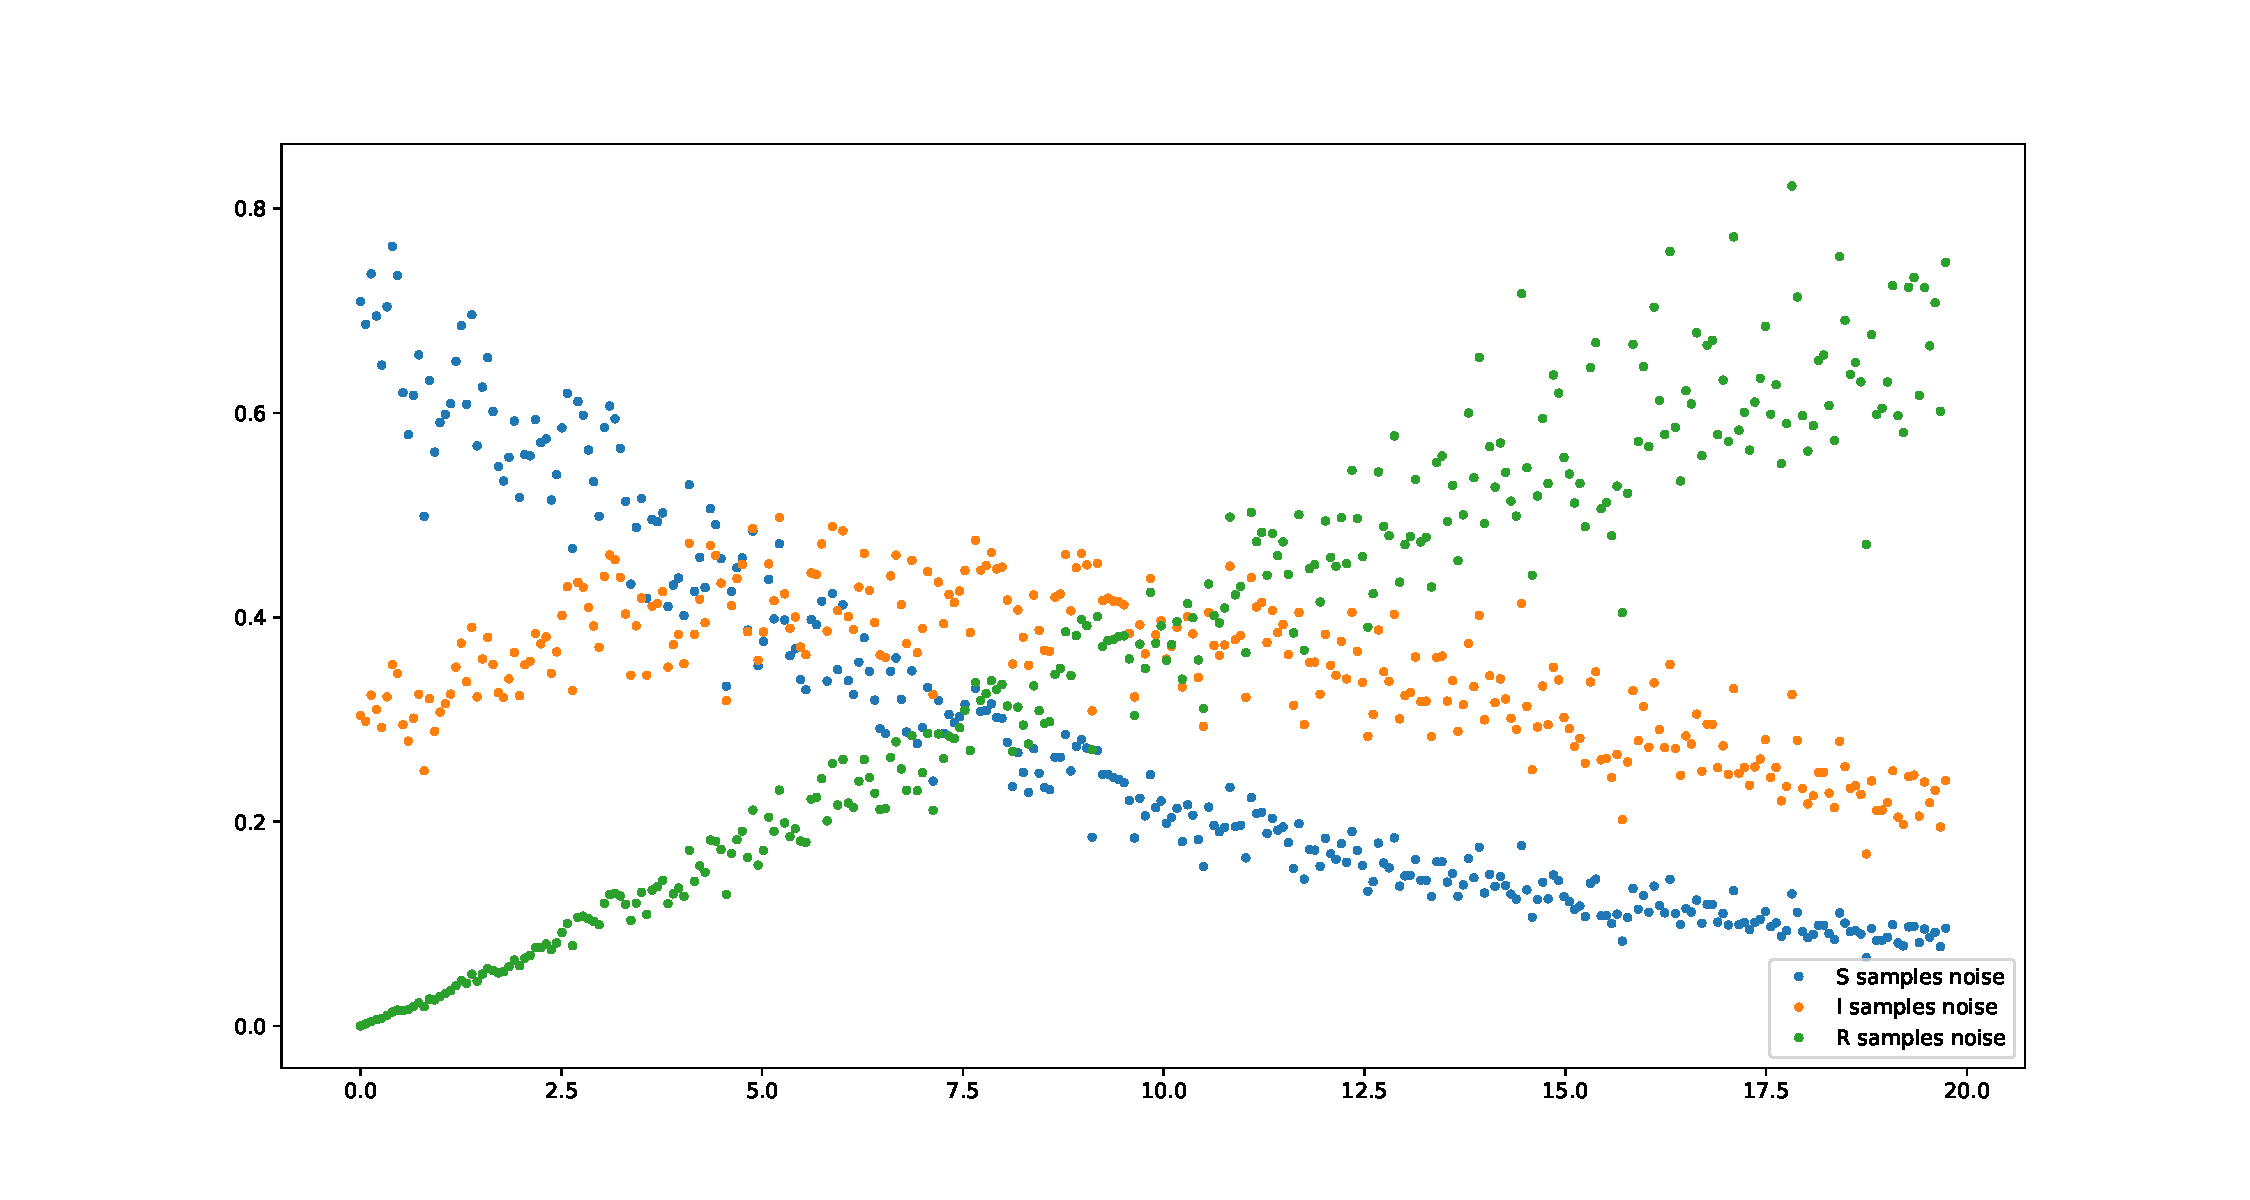
\includegraphics[width=\textwidth]{"figures/SIR_with_noise.pdf"}
    \caption{modelo poblacional SIR con $a = 0.0003, b = 0.1$ y ruido del $10\%$.}
    \label{fig:SIR_with_noise}
\end{figure}

Estos datos son suavizados utilizando un Smoothing Spline en el que se varía su valor de suavizado para cada una de las variables. Por ejemplo, si se suavizan los datos anteriores utilizando un smoothing spline cúbico se obtendrían las curvas que aparecen en la imagen \ref{fig:SIR_noise_with_spline}.

\begin{figure}[h]
    \centering
    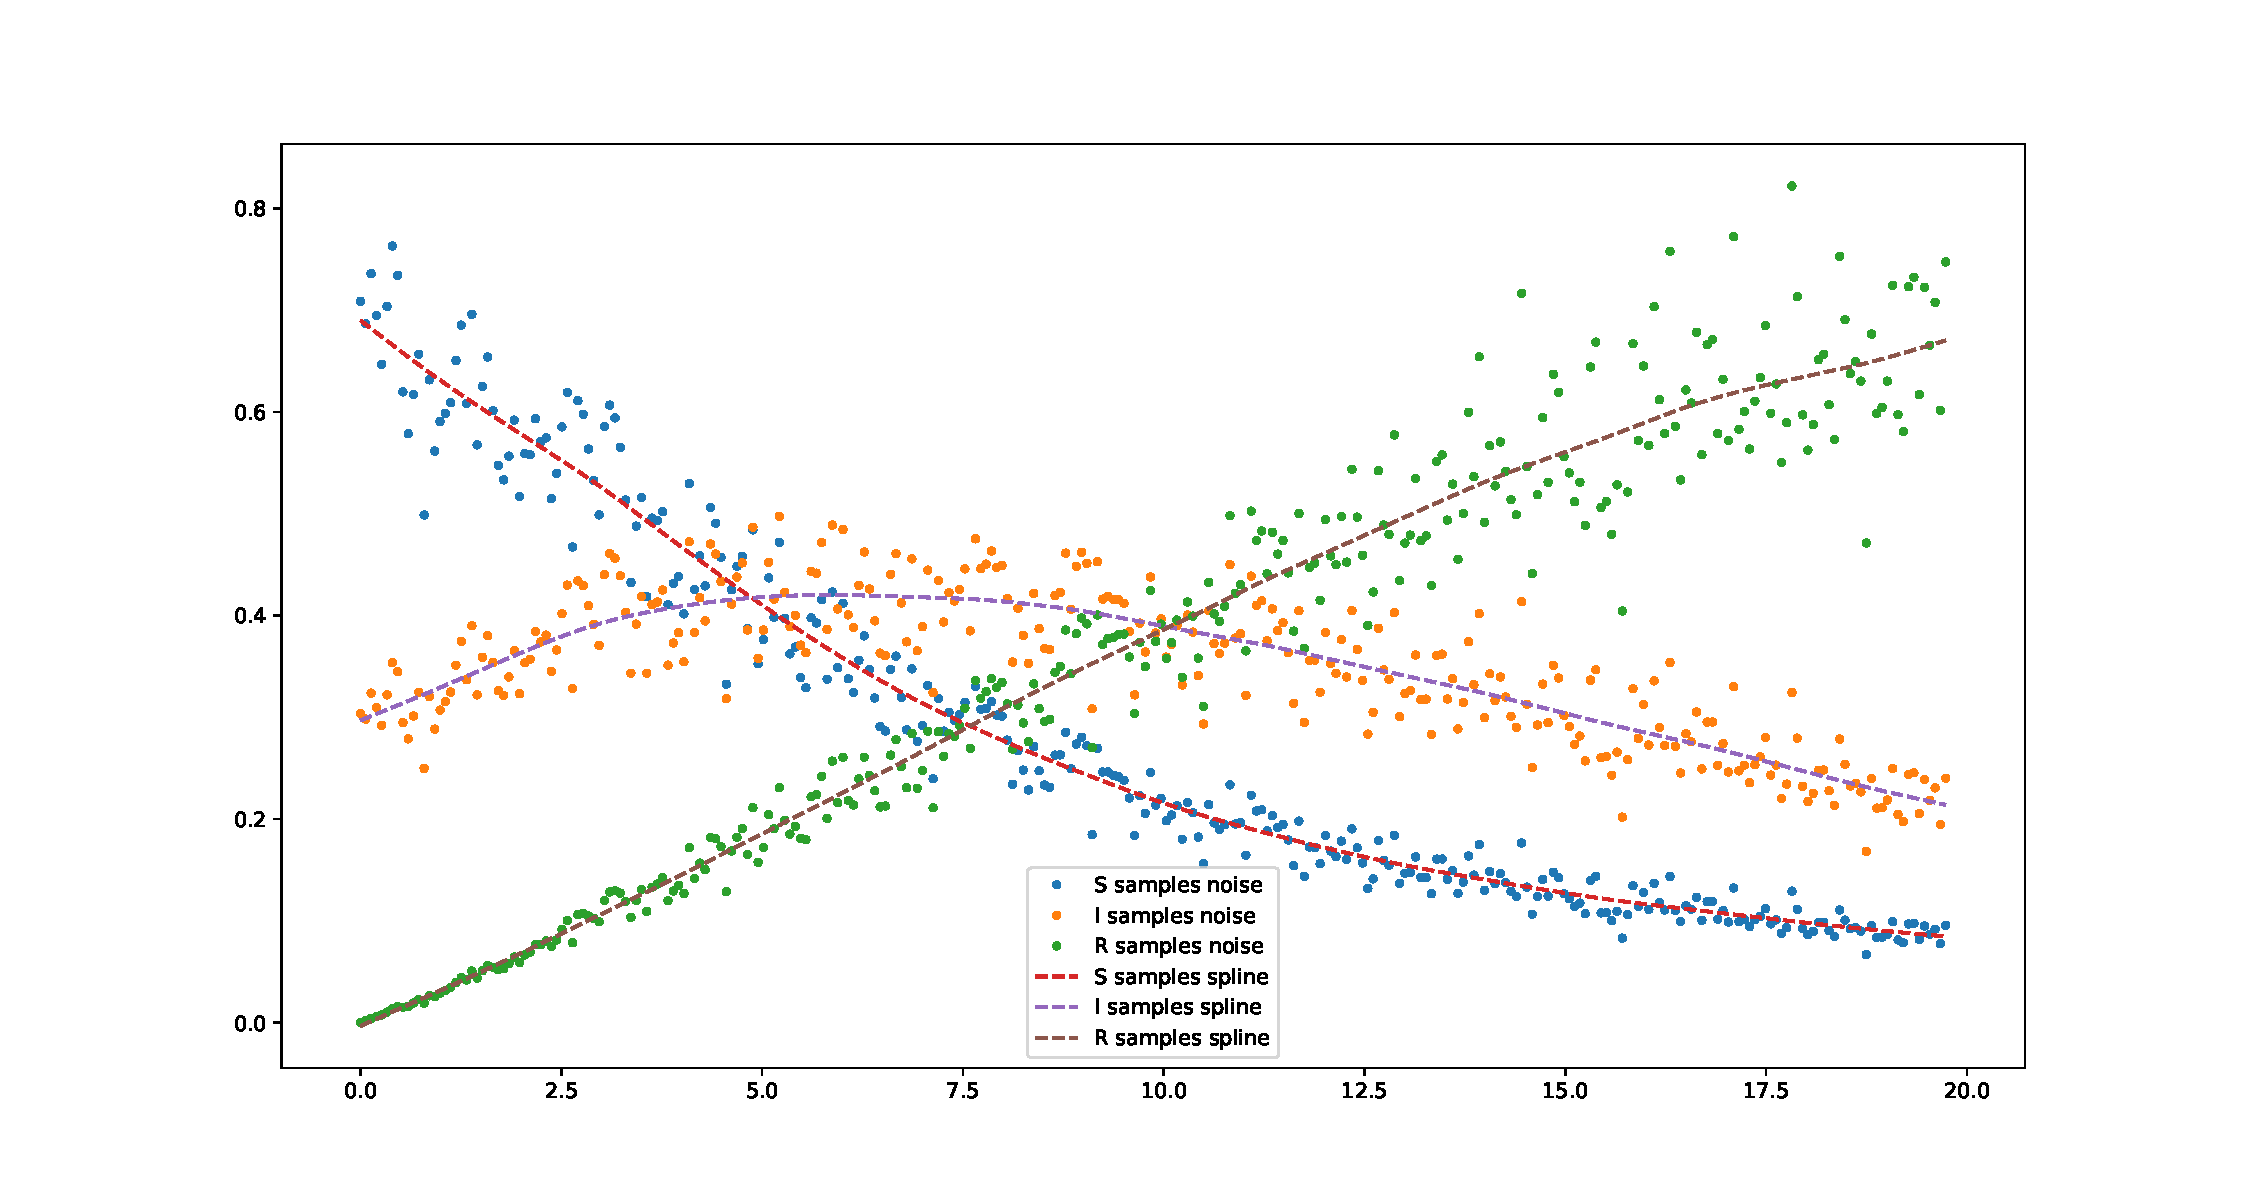
\includegraphics[width=\textwidth]{"figures/SIR_noise_with_spline.pdf"}
    \caption{modelo poblacional SIR con $a = 0.0003, b = 0.1$, ruido del $10\%$ y smoothing-spline con valor de suavizado de $0.1$.}
    \label{fig:SIR_noise_with_spline}
\end{figure}

Una vez que se tiene la función que define el spline de cada variable, se obtiene el valor de la primera derivada de cada una de ellas en distintos instantes de tiempo. Esto permite obtener una aproximación del valor del modelo original en ese instante de tiempo. Por ejemplo retomando el modelo SIR:

\begin{align*}
    S'(t, S, I, R) & \approx spline_S'(t)  \\
    I'(t, S, I, R) & \approx spline_I'(t)  \\
    R'(t, S, I, R) & \approx spline_R'(t).
\end{align*}

Estas aproximaciones de las derivadas de las variables en distintos instantes de tiempo son las que se utilizan en el método de regresión simbólica para encontrar el sistema de ecuaciones diferenciales lineales en los parámetros. Los puntos que se le pasan como datos a la regresión simbólica son igualmente espaciados a lo largo de todo el intervalo de $t$.

Con el propósito de evidenciar las consideraciones expuestas en \ref{section:experimental_considerations} y la descripción de esta sección, se presentan a continuación una serie de experimentos realizados.

\section{Experimentos realizados}\label{section:experiments}

Todos los sistemas de ecuaciones diferenciales seleccionados son sistemas poblacionales lineales en los parámetros. La cantidad de variables en cada uno de estos modelos es distinta y va aumentando con respecto se avanza en el números del experimento.

\subsection{Lotka-Volterra}

El modelo de Lotka-Volterra está definido por el sistema:

\begin{align*}
    X' & = X * (a - b * Y)   \\
    Y' & = -Y * (c - d * X).
\end{align*}

Se utilizaron como valores de los parámetros $a = 0.04$, $b = 0.0005$, $c = 0.2$ y $d = 0.004$ con punto inicial $(20, 20)$ y se integró en el intervalo $0 \leq t \leq 300$ para obtener los datos que aparecen en la figura \ref{fig:lotka_volterra}. De este conjunto de puntos se seleccionaron 300 muestras como datos para el método de regresión simbólica.

\begin{figure}[h]
    \centering
    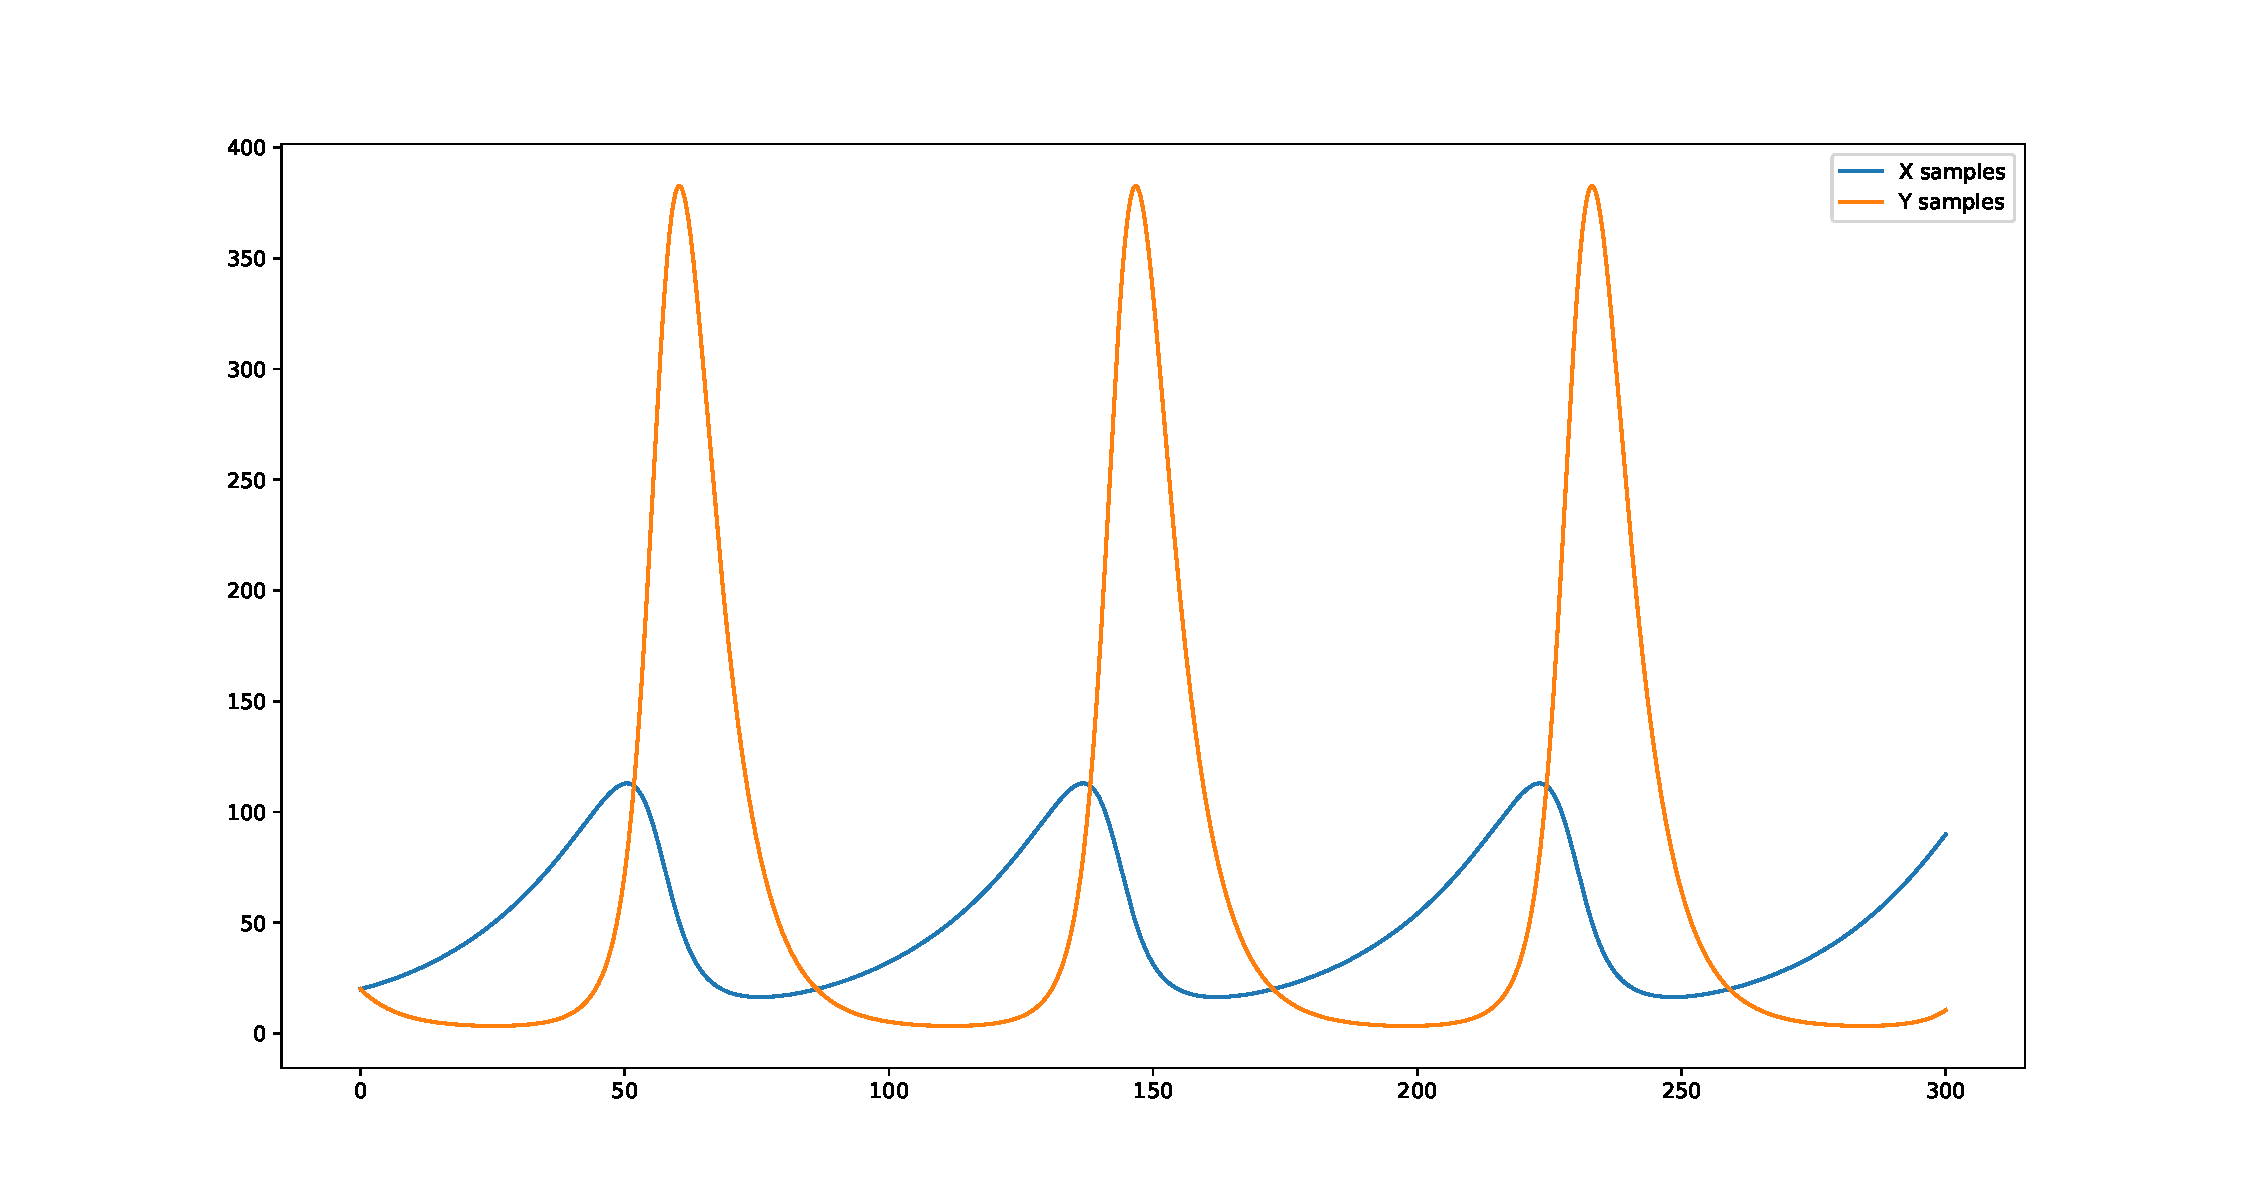
\includegraphics[width=\textwidth]{"figures/lotka_volterra.pdf"}
    \caption{modelo Lotka Volterra con $a = 0.04$, $b = 0.0005$, $c = 0.2$ y $d = 0.004$.}
    \label{fig:lotka_volterra}
\end{figure}

Los resultados obtenidos durante las 30 ejecuciones del experimento aparecen en la tabla \ref{table:experiment_lotka_volterra}.

\begin{table}[!h]
    \centering
    \caption{Resultado obtenidos en el modelo Lotka-Volterra}
    \begin{tabular}{|c|c|c|c|}
        \hline
               & \textbf{ruido de 0\%} & \textbf{ruido de 5\%} & \textbf{ruido de 10\%} \\
        \hline
        media  & 0.02975               & 0.75848               & 1.07525                \\
        \hline
        mínimo & 0.00076               & 0.52541               & 0.88033                \\
        \hline
        máximo & 0.40304               & 1.2288                & 1.44971                \\
        \hline
    \end{tabular}
    \label{table:experiment_lotka_volterra}
\end{table}


\subsection{SIR}

El modelo poblacional SIR está definido por el sistema:

\begin{align*}
    S' & = - a*I*S     \\
    I' & = a*I*S - b*I \\
    R' & = b*I.
\end{align*}

Se utilizaron como valores de los parámetros $a = 0.0003$ y $b = 0.1$ con punto inicial $(700, 300, 0)$ y se integró en el intervalo $0 \leq t \leq 20$ para obtener los datos que aparecen en la imagen \ref{fig:SIR}. De este conjunto de puntos se seleccionaron 300 muestras como datos para el método de regresión simbólica.

Los resultados obtenidos durante las 30 ejecuciones del experimento aparecen en la tabla \ref{table:experiment_SIR}.

\begin{table}[!h]
    \centering
    \caption{Resultado obtenidos en el modelo SIR}
    \begin{tabular}{|c|c|c|c|}
        \hline
               & \textbf{ruido de 0\%} & \textbf{ruido de 5\%} & \textbf{ruido de 10\%} \\
        \hline
        media  & 0.00041               & 7.21204               & 7.46819                \\
        \hline
        mínimo & 0.00029               & 0.79521               & 1.44528                \\
        \hline
        máximo & 0.00144               & 31.77664              & 51.60785               \\
        \hline
    \end{tabular}
    \label{table:experiment_SIR}
\end{table}



\subsection{SIRD}

El modelo poblacional SIRD está definido por el sistema:

\begin{align*}
    S' & = a - b * \frac{S * I}{S + I + R}             \\
    I' & = b * \frac{S * I}{S + I + R} - c * I - d * I \\
    R' & = c * I                                       \\
    D' & = d * I
\end{align*}

Se utilizaron como valores de los parámetros $a = 250$, $b = 0.5$, $c = 0.1$ y $d = 0.2$ con punto inicial $(7000, 3000, 0, 0)$ y se integró en el intervalo $0 \leq t \leq 20$ para obtener los datos que aparecen en la figura \ref{fig:SIRD}. De este conjunto de puntos se seleccionaron 300 muestras como datos para el método de regresión simbólica.

\begin{figure}[h]
    \centering
    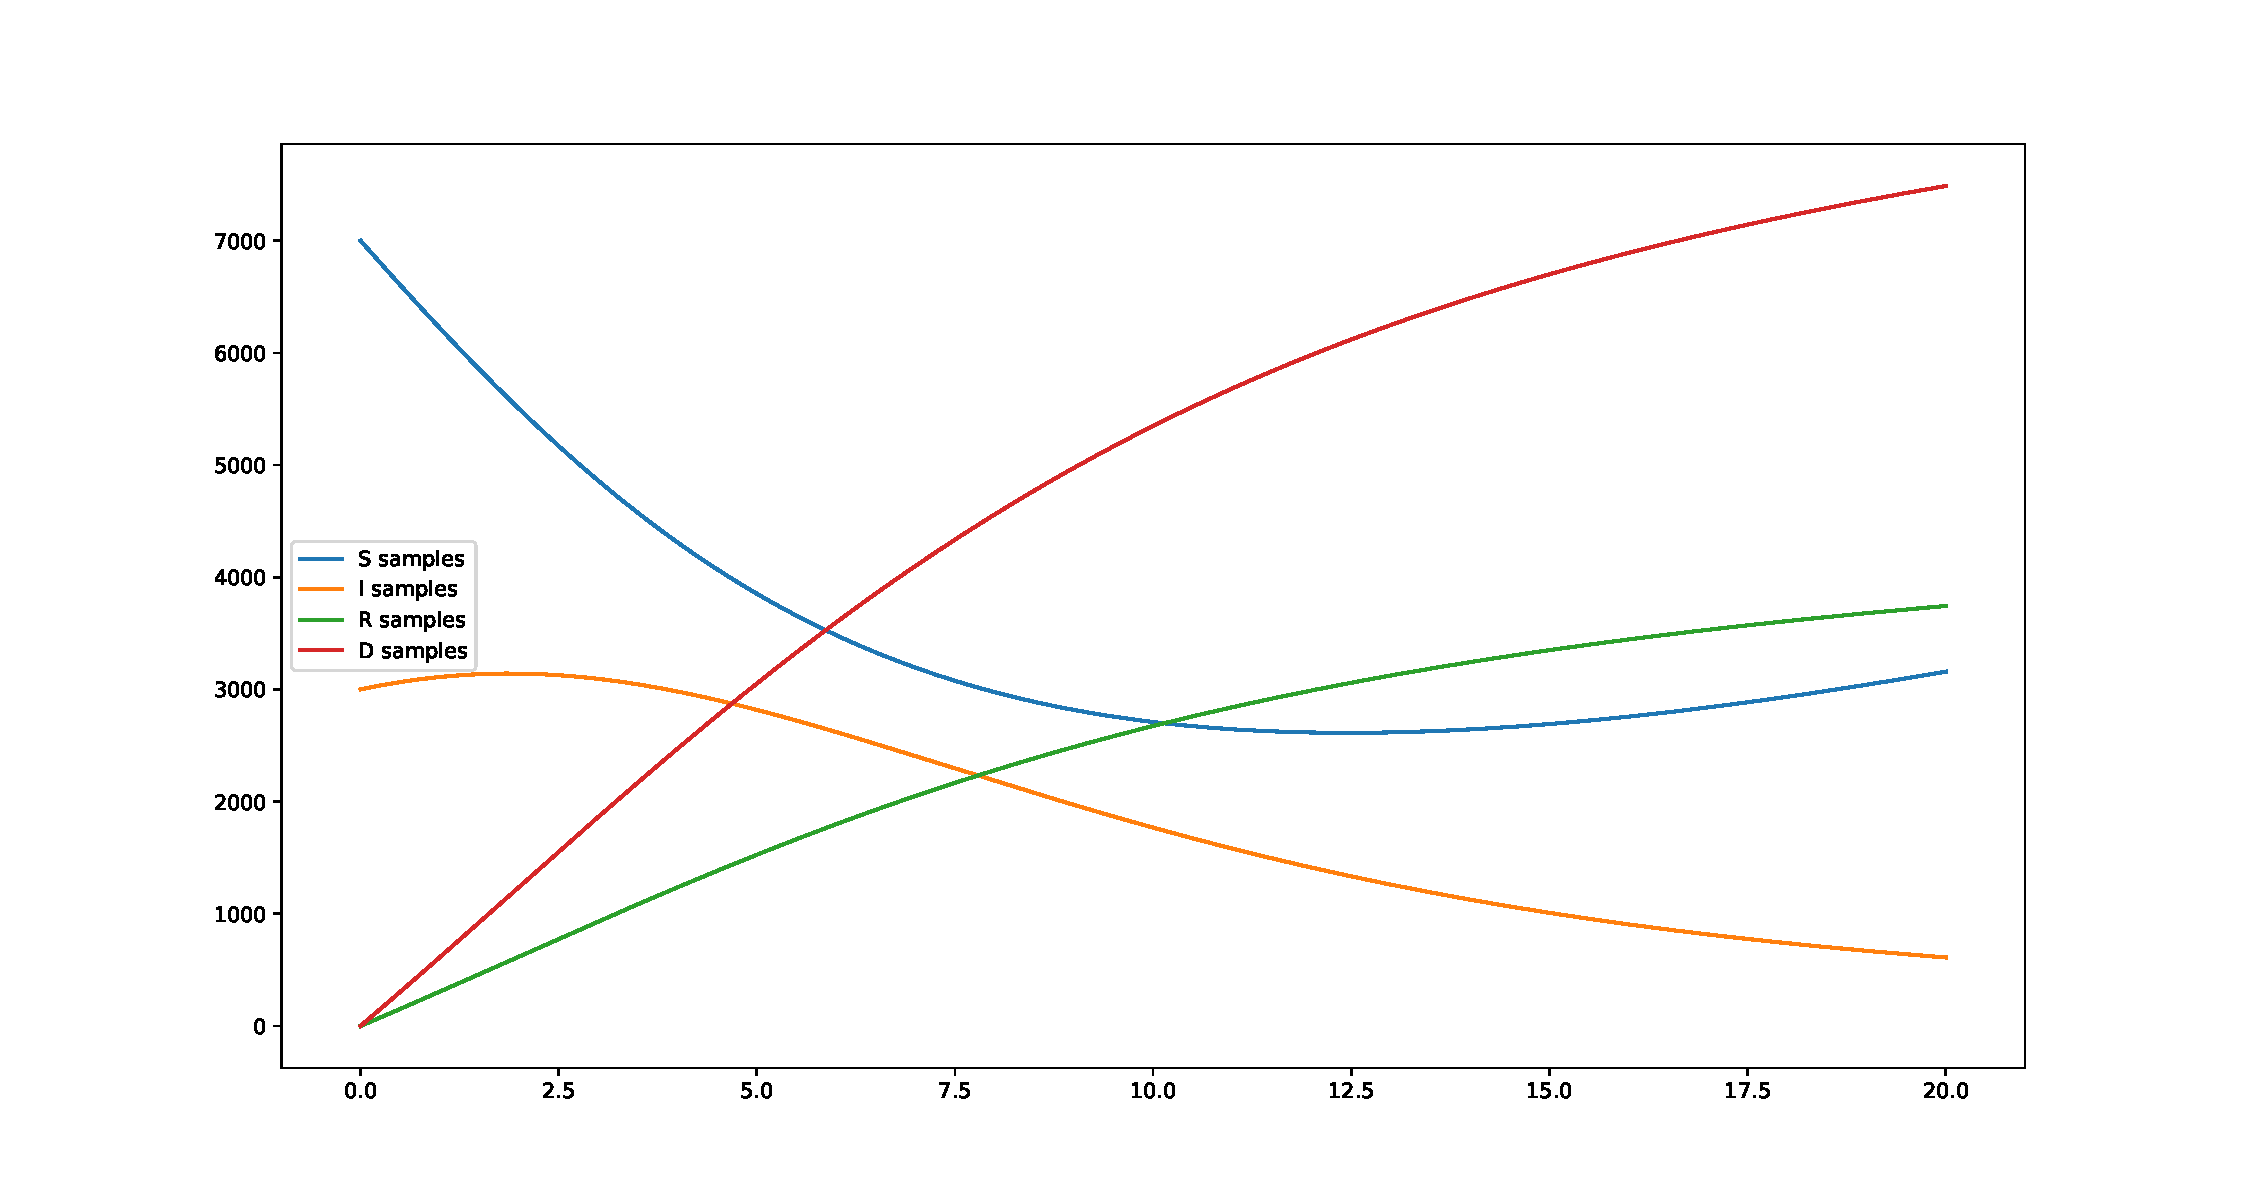
\includegraphics[width=\textwidth]{"figures/SIRD.pdf"}
    \caption{modelo poblacional SIRD con $a = 250$, $b = 0.5$, $c = 0.1$ y $d = 0.2$.}
    \label{fig:SIRD}
\end{figure}

Los resultados obtenidos durante las 30 ejecuciones del experimento aparecen en la tabla \ref{table:experiment_SIRD}.

\begin{table}[!h]
    \centering
    \caption{Resultado obtenidos en el modelo SIRD}
    \begin{tabular}{|c|c|c|c|}
        \hline
               & \textbf{ruido de 0\%} & \textbf{ruido de 5\%} & \textbf{ruido de 10\%} \\
        \hline
        media  & 30.51028              & 86.67886              & 95.15369               \\
        \hline
        mínimo & 0.00674               & 15.37953              & 16.2027                \\
        \hline
        máximo & 190.37824             & 406.15822             & 1391.16075             \\
        \hline
    \end{tabular}
    \label{table:experiment_SIRD}
\end{table}

\subsection{SIQRD}

El modelo poblacional SIQRD está definido por el sistema:

\begin{align*}
    S' & = -\beta * \frac{S * I}{S + I + Q + R + D} - \alpha * S + \delta * Q \\
    I' & = \beta * \frac{S * I}{S + I + Q + R + D} - \gamma * I - \mu * I     \\
    Q' & = \alpha * S - \delta * Q                                            \\
    R' & = \gamma * I                                                         \\
    D' & = \mu * I
\end{align*}

Se utilizaron como valores de los parámetros $\alpha = 0.2$, $\beta = 0.9$, $\delta = 0.1$, $\gamma = 0.1$ y $\mu = 0.05$ con punto inicial $<5000, 3000, 1000, 0, 0>$ y se integró en el intervalo $0 \leq t \leq 20$ para obtener los datos que aparecen en la imagen \ref{fig:SIQRD}. De este conjunto de puntos se seleccionaron 300 muestras como datos para el método de regresión simbólica.

\begin{figure}[h]
    \centering
    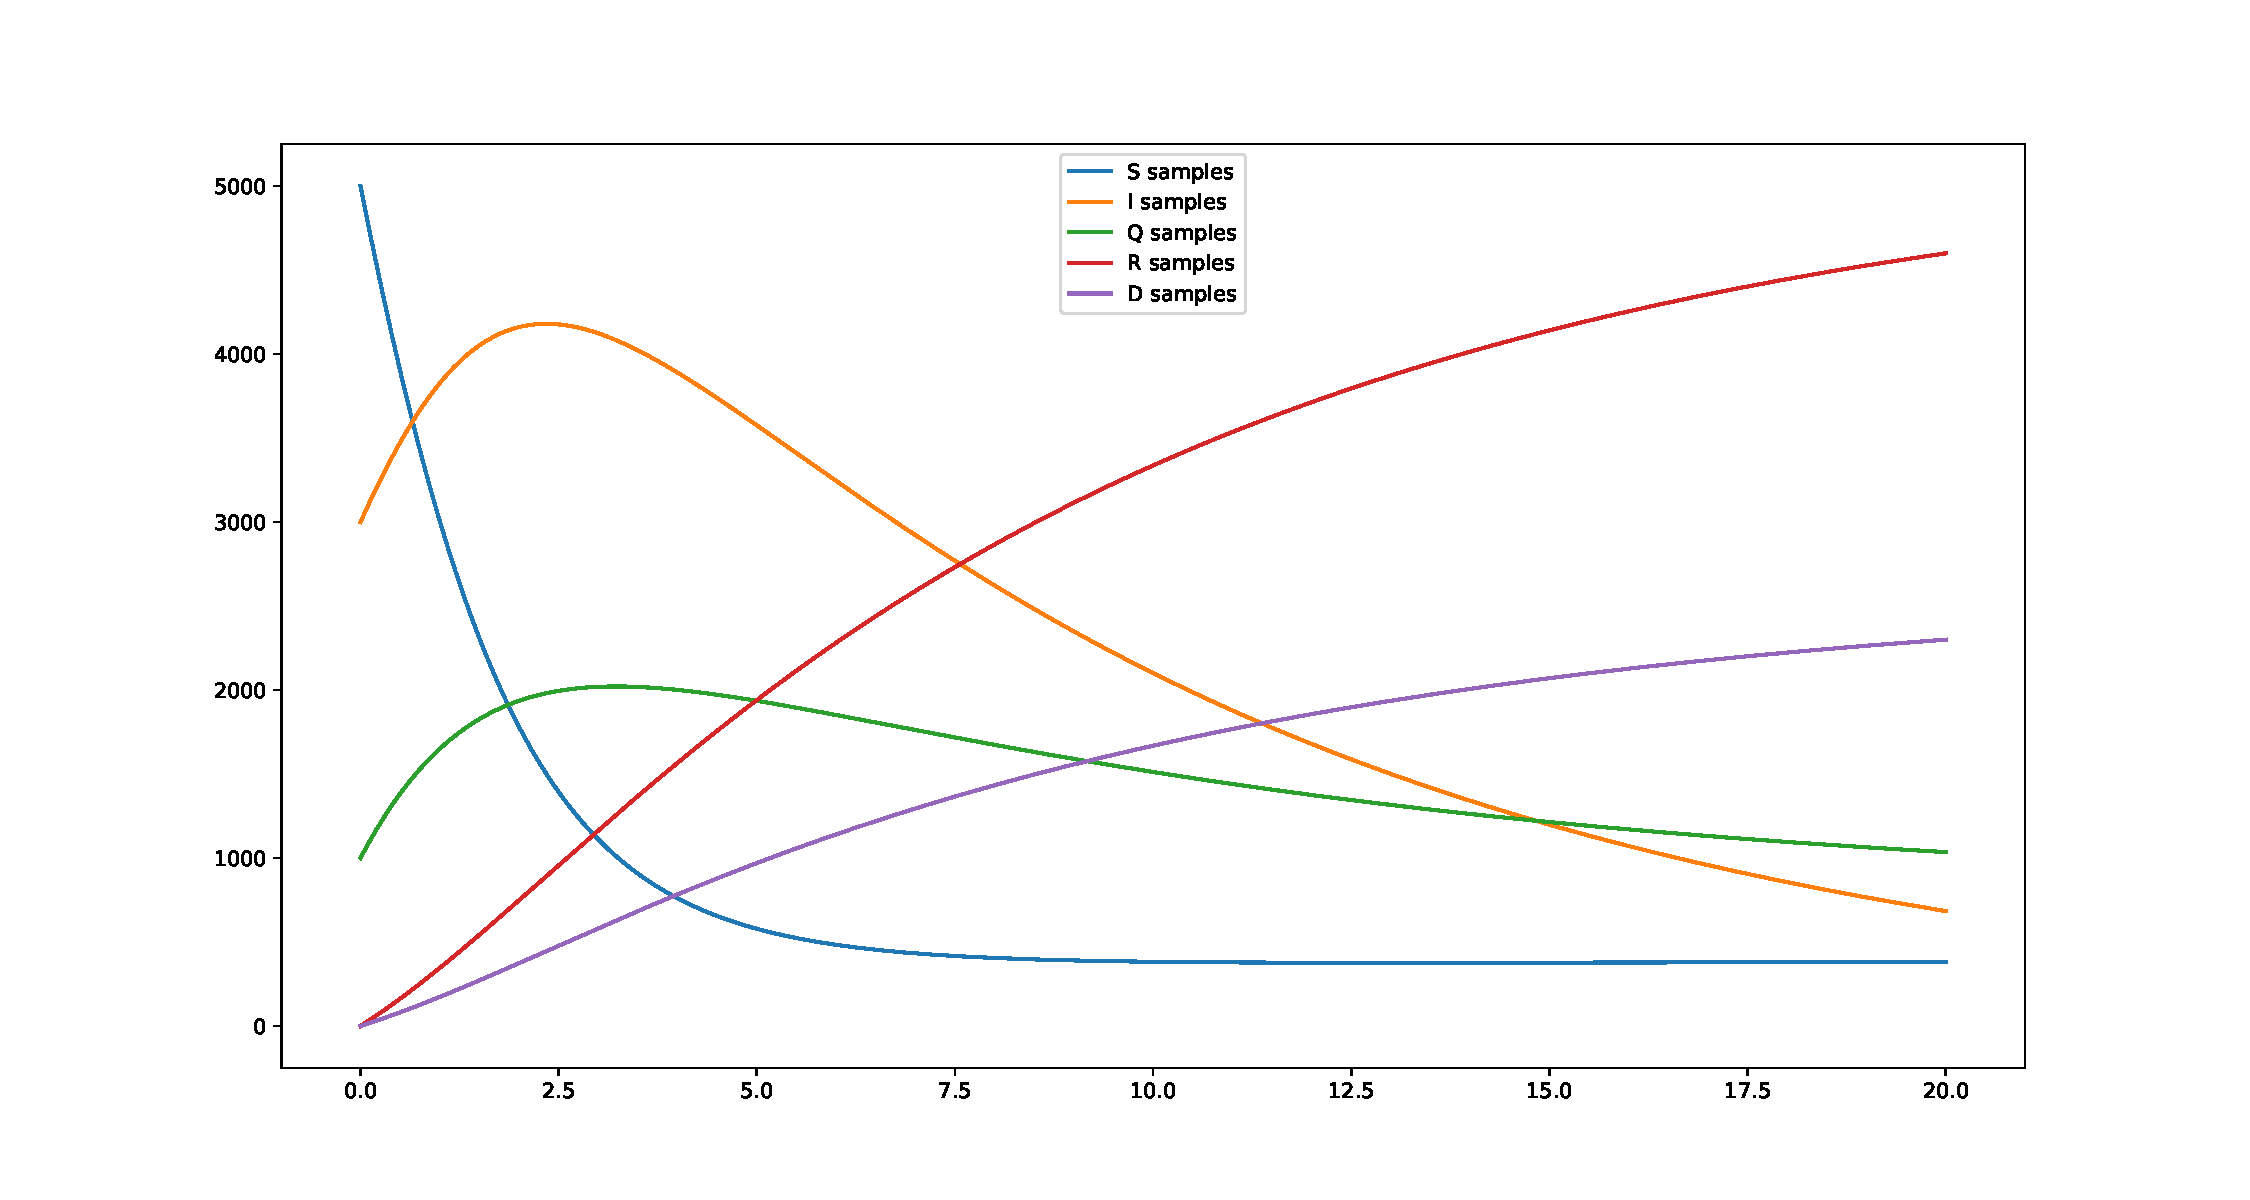
\includegraphics[width=\textwidth]{"figures/SIQRD.pdf"}
    \caption{modelo poblacional SIQRD con $\alpha = 0.2$, $\beta = 0.9$, $\delta = 0.1$, $\gamma = 0.1$ y $\mu = 0.05$.}
    \label{fig:SIQRD}
\end{figure}

Los resultados obtenidos durante las 30 ejecuciones del experimento aparecen en la tabla \ref{table:experiment_SIQRD}.

\begin{table}[!h]
    \centering
    \caption{Resultado obtenidos en el modelo SIQRD}
    \begin{tabular}{|c|c|c|c|}
        \hline
               & \textbf{ruido de 0\%} & \textbf{ruido de 5\%} & \textbf{ruido de 10\%} \\
        \hline
        media  & 5.98884               & 38.34687              & 46.22156               \\
        \hline
        mínimo & 0.1162                & 8.98286               & 12.85924               \\
        \hline
        máximo & 47.14348              & 164.3472              & 259.10153              \\
        \hline
    \end{tabular}
    \label{table:experiment_SIQRD}
\end{table}


\subsection{SVVEIR}

El modelo poblacional SVVEIR está definido por el sistema:

\begin{align*}
    N    & = S + V_1 + V_2 + E + I + R                                        \\
    S'   & = \mu * N - \beta * \frac{I}{N} * S - n * S - \mu * S + \rho * V_1 \\
    V_1' & = n * S - \rho * V_1 - \sigma * V_1 - \mu * V_1                    \\
    V_2' & = \sigma * V_1 - \omega * V_2 - \mu * V_2                          \\
    E'   & = \beta * I / N * S - \alpha * E - \mu * E                         \\
    I'   & = \alpha * E - \gamma * I - \delta * I - \mu * I                   \\
    R'   & = \gamma * I + \omega * V_2 - \mu * R
\end{align*}

Se utilizaron como valores de los parámetros $\alpha = 0.1$, $\beta = 0.7$, $\delta = 0.0005$, $\gamma = 0.05$, $\mu = 0.01$, $n = 0.2$, $\rho = 0.01$, $\omega = 0.05$ y $\sigma = 0.2$ con punto inicial $<5000, 1000, 0, 2000, 1000, 500>$ y se integró en el intervalo $0 \leq t \leq 20$ para obtener los datos que aparecen en la figura \ref{fig:SVVEIR}. De este conjunto de puntos se seleccionaron 300 muestras como datos para el método de regresión simbólica.

\begin{figure}[h]
    \centering
    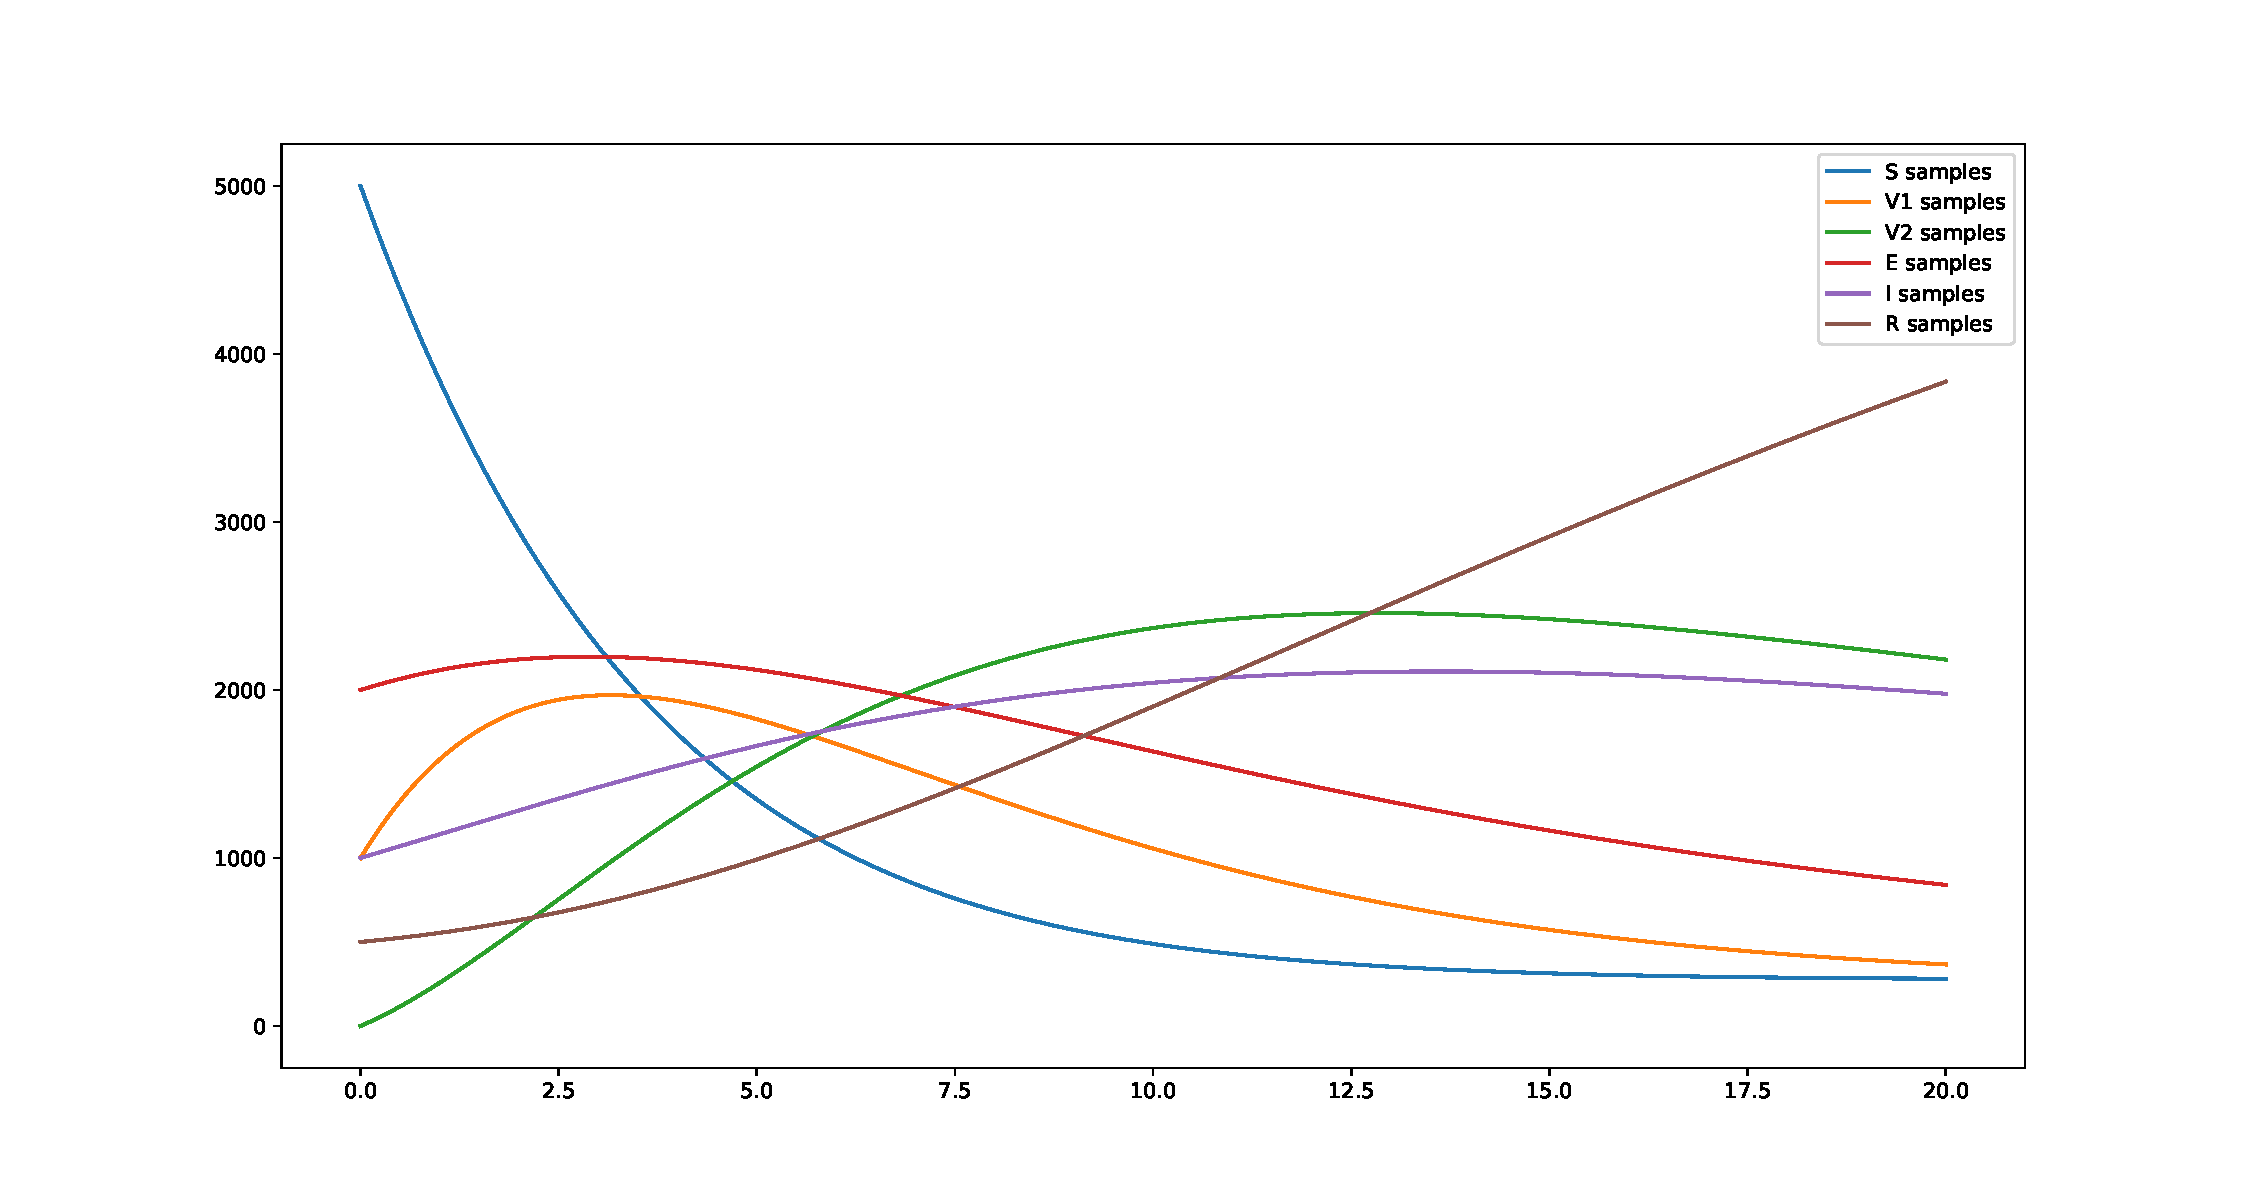
\includegraphics[width=\textwidth]{"figures/SVVEIR.pdf"}
    \caption{modelo poblacional SVVEIR con $\alpha = 0.1$, $\beta = 0.7$, $\delta = 0.0005$, $\gamma = 0.05$, $\mu = 0.01$, $n = 0.2$, $\rho = 0.01$, $\omega = 0.05$ y $\sigma = 0.2$.}
    \label{fig:SVVEIR}
\end{figure}

Los resultados obtenidos durante las 30 ejecuciones del experimento aparecen en la tabla \ref{table:experiment_SVVEIR}.

\begin{table}[!h]
    \centering
    \caption{Resultado obtenidos en el modelo SVVEIR}
    \begin{tabular}{|c|c|c|c|}
        \hline
               & \textbf{ruido de 0\%} & \textbf{ruido de 5\%} & \textbf{ruido de 10\%} \\
        \hline
        media  & 2.59243               & 12.10077              & 19.24528               \\
        \hline
        mínimo & 1.15527               & 9.73051               & 13.38239               \\
        \hline
        máximo & 10.79906              & 28.22324              & 52.39978               \\
        \hline
    \end{tabular}
    \label{table:experiment_SVVEIR}
\end{table}

\section{Análisis de resultados}

Y aquí deberían ir los Análisis de los resultados :D que no se que tal están :'(